\documentclass[11pt]{article}
\usepackage[a4paper, margin=1in]{geometry}
\usepackage{tikz}
\usepackage{amsmath}
\usepackage{lmodern}
\usepackage{bm}
\usepackage{fancyhdr}
\usepackage{amsfonts}
\usepackage{amssymb}
\usepackage{pgfplots}
\usepackage{pgfmath}
\usepackage{lastpage}
\usetikzlibrary{automata, positioning}
\pgfplotsset{compat=1.17}

\title{\textbf{CITS2211 Assignment 2}}
\author{Name: Baasil Siddiqui \\ Student Id: 23895849}
\date{}

\pagestyle{fancy}
\fancyhf{}

\fancyfoot[R]{Page \thepage\ of \pageref{LastPage}}

\begin{document}
\parskip 2mm
\maketitle
\thispagestyle{empty}

\section*{Question 1}
\subsection*{a)}
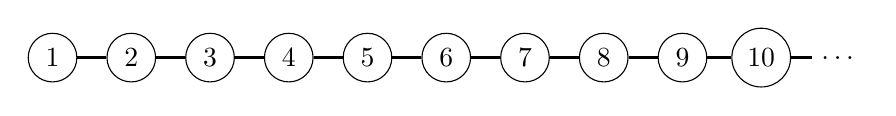
\begin{tikzpicture}
    \node[draw, circle] (top) at (0,0) {$1$};
    \node[draw, circle] [right of=top] (right) {$2$};
    \node[draw, circle] [right of=right] (rtr) {$3$};
    \node[draw, circle] [right of=rtr] (rtrr) {$4$};
    \node[draw, circle] [right of=rtrr] (rtrrr) {$5$};
    \node[draw, circle] [right of=rtrrr] (bottom) {$6$};
    \node[draw, circle] [right of=bottom] (bottom2) {$7$};
    \node[draw, circle] [right of=bottom2] (bottom3) {$8$};
    \node[draw, circle] [right of=bottom3] (bottom4) {$9$};
    \node[draw, circle] [right of=bottom4] (bottom5) {$10$};
    \node [right of=bottom5] (dots) {$\dots$};
    \draw[thick] (top) -- (right) -- (rtr) -- (rtrr) -- (rtrrr) --
          (bottom) -- (bottom2) -- (bottom3) -- (bottom4) --
          (bottom5) -- (dots);
\end{tikzpicture}

\subsection*{b)}

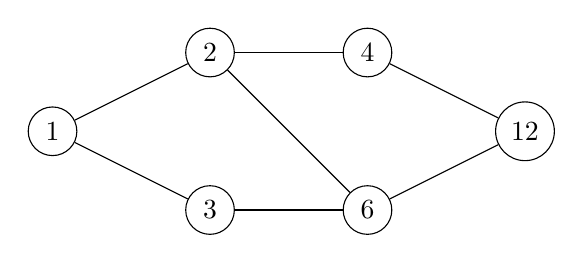
\begin{tikzpicture}
    \node[draw, circle] (one) at (0,0) {$1$};
    \node[draw, circle] (two) at (2,1) {$2$};
    \node[draw, circle] (three) at (2,-1) {$3$};
    \node[draw, circle] (four) at (4,1) {$4$};
    \node[draw, circle] (six) at (4,-1) {$6$};
    \node[draw, circle] (twelve) at (6,0) {$12$};

    \draw (one) -- (two);
    \draw (one) -- (three);
    \draw (two) -- (four);
    \draw (two) -- (six);
    \draw (three) -- (six);
    \draw (four) -- (twelve);
    \draw (six) -- (twelve);
\end{tikzpicture}

\subsection*{c)}

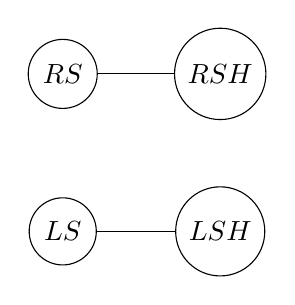
\begin{tikzpicture}
    \node[draw, circle] (rs) at (0,1) {$RS$};
    \node[draw, circle] (ls) at (0,-1) {$LS$};
    \node[draw, circle] (rsh) at (2,1) {$RSH$};
    \node[draw, circle] (lsh) at (2,-1) {$LSH$};

    \draw (rs) -- (rsh);
    \draw (ls) -- (lsh);
\end{tikzpicture}

\section*{Question 2}
\subsection*{a)}

the relation is reflexive if $\forall x \in \mathbb{R} ((x,  x) \in R)$ \\
subtrating any real number by itself results in zero which is an integer, Hence
R is reflexive. \\
\\
The relation is symmetric if for all $(x, y) \in R$, $(y, x) \in R$ if $x \neq y$
we need to show that if x - y is an integer, y - x is an integer as well
%
\begin{align*}
    \text{let } x - y &= k \text{ where } x \in \mathbb{Z} \\
    y - x &= -k  \text{ (arithmetic)}
\end{align*}
%
k is an integer so -k is an integer as \\
hence, y - x is an integer \\
Therefore, we have proved that is $(x, y) \in R$ then $(y, x) \in R$
and relation R is symmetric
\\
The relation R is transitive if for all $x, y, z \in \mathbb{R}$ if xRy and yRz then xRz holds \\
so we need to prove that if $x - y \in \mathbb{Z}$ and $y - z \in \mathbb{Z}$ then $x - z \in \mathbb{Z}$
%
\begin{align*}
    \text{let } x - y &= k_{1} \text{ where $k_{1}$ is an integer} \\
    \text{let } y - z &= k_{2} \text{ where $k_{2}$ is an integer} \\
    x - z &= (x - y) + (y - z) \text{  (adding and substracting y)} \\
    &= k_{1} + k_{2}
\end{align*}
both $k_{1}$ and $k_{2}$ are integers so $k_{1} + k_{2}$ is integer as well,
so x - z is an integer and $(x, z) \in R$ and the relation R is transitive \\
\\
Q.E.D.

\subsection*{b)}
\textbf{i.} \\
the equivalence class of any real number x is given by \\
$[x] = \{y \in \mathbb{R} \;|\; y - x \in \mathbb{Z}\}$ \\
let y - x be an integer k then y = x + k \\
Therefore, the equivalence class of any real number x consists of all numbers
produced by adding an integer to x
since the numbers integers is infinite, each equivalence class is infinite
\\ \\
\textbf{ii.} \\
as proved in part \textbf{i} every real number has an equivalence classes therefore,
the total number of equivalence classes are infinite.

\section*{Question 3}
Assume a new generation starts every 40 years \\
We have 50 generations in 2000 years so the person should have $2^{50}$ ancestors 2000 years ago
the current poopulation is less than 8 billion which is $2^3 \times 10^9 = 2^{12} \times 5^9$
which is less than $2^{39}$ \\
the population has only increased so the population
2000 years ago was certainly less than $2^{50}$ \\
by pigeonhole principle at least two ancestors of the person were the
same person \\
Q.E.D.


\section*{Question 4}
\subsection*{a)}
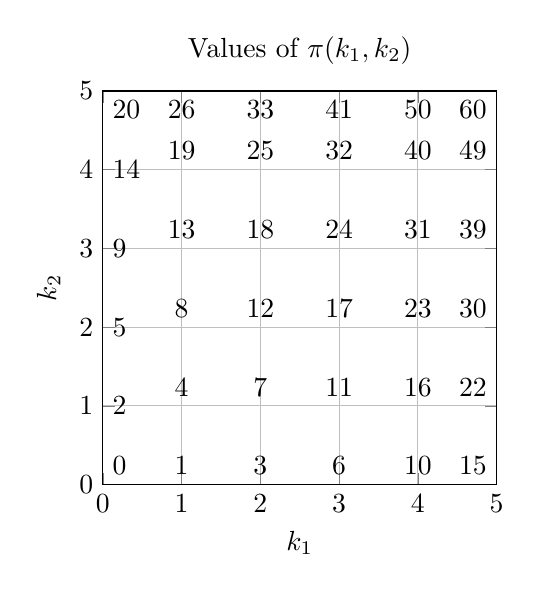
\begin{tikzpicture}
    \begin{axis}
    [
        x=1cm,
        y = 1cm,
        xlabel={$k_1$},
        ylabel={$k_2$},
        title={Values of $\pi(k_1, k_2)$},
        ymin=0,
        ymax=5,
        xmin=0,
        xmax=5,
        xtick={0,1,2,3,4,5},
        ytick={0,1,2,3,4,5},
        grid = major
    ]

        \node at (axis cs:0,0) [anchor=south west] {$0$};
        \node at (axis cs:0,1) [anchor=west] {$2$};
        \node at (axis cs:0,2) [anchor=west] {$5$};
        \node at (axis cs:0,3) [anchor=west] {$9$};
        \node at (axis cs:0,4) [anchor=west] {$14$};
        \node at (axis cs:0,5) [anchor=north west] {$20$};

        \node at (axis cs:1,0) [anchor=south] {$1$};
        \node at (axis cs:1,1) [anchor=south] {$4$};
        \node at (axis cs:1,2) [anchor=south] {$8$};
        \node at (axis cs:1,3) [anchor=south] {$13$};
        \node at (axis cs:1,4) [anchor=south] {$19$};
        \node at (axis cs:1,5) [anchor=north] {$26$};

        \node at (axis cs:2,0) [anchor=south] {$3$};
        \node at (axis cs:2,1) [anchor=south] {$7$};
        \node at (axis cs:2,2) [anchor=south] {$12$};
        \node at (axis cs:2,3) [anchor=south] {$18$};
        \node at (axis cs:2,4) [anchor=south] {$25$};
        \node at (axis cs:2,5) [anchor=north] {$33$};

        \node at (axis cs:3,0) [anchor=south] {$6$};
        \node at (axis cs:3,1) [anchor=south] {$11$};
        \node at (axis cs:3,2) [anchor=south] {$17$};
        \node at (axis cs:3,3) [anchor=south] {$24$};
        \node at (axis cs:3,4) [anchor=south] {$32$};
        \node at (axis cs:3,5) [anchor=north] {$41$};

        \node at (axis cs:4,0) [anchor=south] {$10$};
        \node at (axis cs:4,1) [anchor=south] {$16$};
        \node at (axis cs:4,2) [anchor=south] {$23$};
        \node at (axis cs:4,3) [anchor=south] {$31$};
        \node at (axis cs:4,4) [anchor=south] {$40$};
        \node at (axis cs:4,5) [anchor=north] {$50$};

        \node at (axis cs:5,0) [anchor=south east] {$15$};
        \node at (axis cs:5,1) [anchor=south east] {$22$};
        \node at (axis cs:5,2) [anchor=south east] {$30$};
        \node at (axis cs:5,3) [anchor=south east] {$39$};
        \node at (axis cs:5,4) [anchor=south east] {$49$};
        \node at (axis cs:5,5) [anchor=north east] {$60$};
    \end{axis}
\end{tikzpicture}

\subsection*{b)}
The function $\pi$ is bijection between $\mathbb{N}^2$ and $\mathbb{N}$.
We need to prove that there exists a bijection between $\mathbb{N}^n$ and $\mathbb{N}$ \\
We will prove this using induction \\
let $P(k)$ be $|\mathbb{N}^k| = |\mathbb{N}|$ \\
\\
\textbf{\underline{Base case:}} The base case is n = 1 \\
$\mathbb{N}^1 = \mathbb{N}$ \\
$|\mathbb{N}| = |\mathbb{N}|$ is trivially true \\
\\
\textbf{\underline{Inductive Case:}} \\
We need to prove that $P(k) \rightarrow P(k+1)$ for some arbitary $k \geq 1$ \\
\\
\textbf{Inductive hypothesis:} \\
We can assume that $P(k)$ holds for an arbitary $k \geq 1$ \\
\\
\textbf{Inductive step:} \\
now we need to show that $P(k+1)$ holds given $P(k)$ is true \\
we know that there is a bijection f from $\mathbb{N}^n$ to $\mathbb{N}$ from
the inductive hypothesis \\
So, $\mathbb{N}^n$ can be mapped to a single natural number
$\mathbb{N}^{n+1}$ can be written as $\mathbb{N}^n \times \mathbb{N}$ \\
$\mathbb{N}^n \times \mathbb{N}$ can further be mapped using the function $\pi$ \\
since we know that both $\pi$ and $f$ function are bijections, they can be
combined to a single bijective function from $\mathbb{N}^{n+1}$ to $\mathbb{N}$ \\
Therefore, $|\mathbb{N}^{n+1}| = |\mathbb{N}|$ \\
Q.E.D.


\section*{Question 5}
We need to prove that a bijection from $B$ to $A^B$ doesn't exist \\
assume a bijection f from $B$ to $A^B$ exists \\
for every $x \in B$, $f(x) \in A^B$. f(x) is a function from B to A. \\
Now, we can define new function $f^\prime$ such that
$f^\prime (x) \neq (f(x))(x)$ \\
since, $|A| \geq 2$ we can define this function by choosing a different value from set
$A$ for every value of $x \in B$ (using the diagonal argument) \\
the function f is a bijection so there must be some value of $x \in B$ such that
$f(x) = f^\prime$ \\
\\
This contradicts with the definition of $f^\prime$ function since this would imply
that $f(x)(y) = f^\prime(y)$ for all $y \in B$ \\
our assumption that f is a bijection must be false
Therefore, a bijection from set $B$ to $A^B$ doesn't exist and $|A^B| \neq |B|$. \\
Q.E.D.

\section*{Question 6}
\subsection*{a)}
\textbf{States:} $Q = \{q_1, q_2, q_3\}$ \\
\textbf{Start state:} $q_0 = q_1$ \\
\textbf{Alphabet:} $\Sigma = \{0, 1\}$ \\
\textbf{Accepting states:} $F = \{q_1, q_3\}$ \\
\textbf{State transition:} $\delta : Q \times \Sigma -> \mathcal{P}(Q)$ \\

\subsection*{b)}
FSM recognises the symbols 1 and 0
\begin{itemize}
    \item $q_1$ is the starting state and it stays there if it reads 0 and moves to $q_2$ if it reads 1
    \item in state $q_2$ it doesn't move if it reads 0 and moves to $q_3$ if it reads 1
    \item in state $q_3$ it only accepts the symbol 0 and stays in $q_3$
\end{itemize}
states $q_1$ and $q_3$ are the accepting states \\
Thus, the FSM accepts strings that contain exactly two 1s and any number of 0s including none anywhere

\subsection*{c)}
0*10*10*

\section*{Question 7}
\textbf{States:} \\
set of States of the DFSM is the powerset of the states of the original NFSM \\
$Q = \{\phi, \{q_0\}, \{q_1\}, \{q_0, q_1\}\}$ \\
\\
\textbf{Initial state:} \\
The initial state of the DFSM is a singleton set containing the initial state of the NFSM \\
$\{q_0\}$ is the initial state \\
\\
\textbf{Accepting states:} \\
accepting states of the DFSM are the states containing any accepting states of NFSM \\
$\{q_1\}$ and $\{q_0, q_1\}$ are the accepting states \\
\\
\textbf{The Transition Function:} \\
The transition function, $\delta$ , returns the union of all states that are
reachable via the original transition function $\delta'$ , by consuming the
input from any of the NFSM states in the current DFSM state, i.e.,
$\delta(s, x) = \bigcup \{ \delta'(q, x) \mid q \in s \}$

The Result could be simpliefied by removing the state $\{q_1\}$ since there is no way
to reach the state and it's part of the combined state $\{q_0, q_1\}$

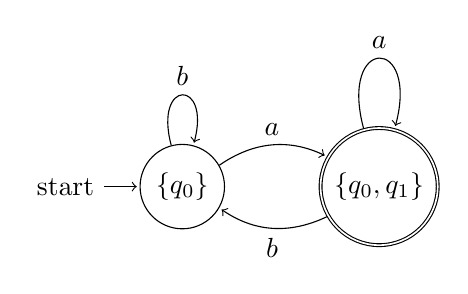
\begin{tikzpicture}[shorten >=1pt, node distance=2.5cm, on grid, auto]
   \node[state, initial] (q0)   {$\{q_0\}$};
   \node[state, accepting, right=of q0] (q0q1) {$\{q_0, q_1\}$};

    \path[->]
    (q0) edge [loop above] node {$b$} ()
          edge [bend left, above] node {$a$} (q0q1)
    (q0q1) edge [bend left, below] node {$b$} (q0)
            edge [loop above] node {$a$} ();
\end{tikzpicture}

\section*{Question 8}
\subsection*{a)}
b*ab*aab*aaab*

\subsection*{b)}
\begin{itemize}
    \item ((11)*)1*)* can be simplified to 1* since (11)* means even number of
          1s and the 1* provides additional 1s which means an empty string
          of any string made of 1s is accepted
    \item (11 + 1)* can be simplified to 1* because 11* would be even number of
        1s and 1* would make any number of 1s including none.
    \item (0 + $\epsilon$)* can be simplified to 0* since $\epsilon$* can be
        covered by no zeroes included in 0*
    \item the expression can be further simplified by combining 1* + 1* to 1*
\end{itemize}
final expression is 1* + 0*

\section*{Question 9}
The claim is similar to the pumping lemma but the pumping length needs to be
different for every language the condition $|w| \ge 1$ is not sufficient for
all languages \\
\\
\textbf{Counter example:} \\
Consider the language (ab)* let's take w as ab, $|w| \ge 1$ so we satisfy the condition \\
if y = a, and i = 2, the resulting string aab is not in the language (ab)* \\
similarly if y = b and i = 2 the resulting string abb is not in the language \\
those are the only two possibilities of y since cardinality of y needs to be greater than 1 \\

\section*{Question 10}
\textbf{a) $\{a^nb^ma^n \;|\; m, n \in \mathbb{N}\}$} \\
\\
The automata reads at least one 'a' and pushes each 'a' read onto the stack. \\
It requires at least one b and doesn't change the stack. \\
Then it requires at least one a and pops a from the stack for every a read.
The PDA accepts if the stack is empty after reading the input. \\
\\
\textbf{a) $\{a^nb^m \;|\; n \leq m \leq 2n \land m, n \in \mathbb{N}\}$} \\
\\
The PDA reads at least one 'a' and pushed each 'a' read onto the stack \\
When it starts reading 'b's it non deterministically chooses whether to pop 'a'
from the stack for each b read or pop 'a' on reading two b's. The automata accepts
if the stack is empty after reading the input. This ensures that for valid strings
there is atleast one path to acceptance and the numebr of b's read is in the range
(n, 2n).

\section*{Question 11}
\textbf{a)} \\
\\
$A \rightarrow 0A \;|\; 1A \;|\; \epsilon $ \\
$S \rightarrow 0A1 \;|\; 1A0 $ \\
\\
if the string starts at 0 then it must end with 1 and vice versa.
within the 1 and 0, A accepts any combination of 1s and 0s \\
\\
\textbf{b)} \\
\\
$A \rightarrow 01A \;|\; 10A \;|\; \epsilon$ \\
$S \rightarrow AS \;|\; SA \;|\; 1$ \\
\\
A has equal number of ones and zeroes and S adds the additional ones.

\end{document}

